\lab{Introduction to Scikit-Learn}{Introduction to Scikit-Learn}
\objective{Scikit-learn is the one of the fundamental tools in Python for machine learning.
In this appendix we highlight and give examples of some popular scikit-learn tools for classification and regression, training and testing, data normalization, and constructing complex models.}

\begin{info}
This guide corresponds to scikit-learn version 0.20, which has a few significant differences from previous releases.
See \url{http://scikit-learn.org/stable/whats_new.html} for current release notes.
Install scikit-learn (the \li{sklearn} module) with \li{conda install scikit-learn}.
\end{info}

% \textbf{Reading}: \url{http://scikit-learn.org/stable/tutorial/index.html}.

\section*{Base Classes and API} % =============================================

Many machine learning problems center on constructing a function $f:X\rightarrow Y$, called a \emph{model} or \emph{estimator}, that accurately represents properties of given data.
The domain $X$ is usually $\mathbb{R}^D$, and the range $Y$ is typically either $\mathbb{R}$ (regression) or a subset of $\mathbb{Z}$ (classification).
The model is trained on $N$ \emph{samples} $(\x_i)_{i=1}^N \subset X$ that usually (but not always) have $N$ accompanying \emph{labels} $(y_i)_{i=1}^N \subset Y$.

Scikit-learn \cite{scikit-learn,sklearn_api} takes a highly object-oriented approach to machine learning models.
Every major scikit-learn class inherits from \li{sklearn.base.BaseEstimator} and conforms to the following conventions:

\begin{enumerate}
\item The constructor \li{__init__()} receives \emph{hyperparameters} for the classifier, which are parameters for the model $f$ that are \textbf{not dependent on data}.
Each hyperparameter must have a default value (i.e., every argument of \li{__init__()} is a keyword argument), and each argument must be saved as an instance variable of the \textbf{same name} as the parameter.

\item The \li{fit()} method constructs the model $f$.
It receives an $N\times D$ matrix $X$ and, optionally, a vector $\y$ with $N$ entries.
Each row $\x_i$ of $X$ is one sample with corresponding label $y_i$.
By convention, \li{fit()} always returns \li{self}.
\end{enumerate}
%
Along with the \li{BaseEstimator} class, there are several other ``mix in'' base classes in \li{sklearn.base} that define specific kinds of models.
The three listed below are the most common.\footnote{See \url{http://scikit-learn.org/stable/modules/classes.html\#base-classes} for the complete list.}

\begin{itemize}
\item \li{ClassifierMixin}: for \emph{classifiers}, estimators that take on discrete values.
\item \li{RegressorMixin}: for \emph{regressors}, estimators that take on continuous values.
\item \li{TransformerMixin}: for preprocessing data before estimation.
\end{itemize}

\subsection*{Classifiers and Regressors} % ------------------------------------

The \li{ClassifierMixin} and \li{RegressorMixin} both require a \li{predict()} method that acts as the actual model $f$.
That is, \li{predict()} receives an $N\times D$ matrix $X$ and returns $N$ predicted labels $(y_i)_{i=1}^N$, where $y_i$ is the label corresponding to the $i$th row of $X$.
Both of these base class have a predefined \li{score()} method that uses \li{predict()} to test the accuracy of the model.
It accepts $N\times D$ test data and a vector of $N$ corresponding labels, then reports either the classification accuracy (for classifiers) or the $R^2$ value of the regression (for regressors).

For example, a \li{KNeighborsClassifier} from \li{sklearn.neighbors} inherits from \li{BaseEstimator} and \li{ClassifierMixin}.
This classifier uses a simple strategy: to classify a new piece of data $\z$, find the $k$ training samples that are ``nearest'' to $\z$, then take the most common label corresponding to those nearest neighbors to be the label for $\z$.
Its constructor accepts hyperparameters such as \li{n_neighbors}, for determining the number of neighbors $k$ to search for, \li{algorithm}, which speficies the strategy to find the neighbors, and \li{n_jobs}, the number of parallel jobs to run during the neighbors search.
Again, these hyperparameters are independent of any data, which is why they are set in the constructor (before fitting the model).
Calling \li{fit()} organizes the data $X$ into a data structure for efficient nearest neighbor searches (determined by \li{algorithm}).
Calling \li{predict()} executes the search, determines the most common label of the neighbors, and returns that label.

\begin{lstlisting}
>>> from sklearn.datasets import load_breast_cancer
>>> from sklearn.neighbors import KNeighborsClassifier
>>> from sklearn.model_selection import train_test_split

# Load the breast cancer dataset and split it into training and testing groups.
>>> cancer = load_breast_cancer()
>>> X_train, X_test, y_train, y_test = train_test_split(cancer.data,
...                                                     cancer.target)
>>> print(X_train.shape, y_train.shape)
(426, 30) (426,)        # There are 426 training points, each with 30 features.

# Train a KNeighborsClassifier object on the training data.
# fit() returns the object, so we can instantiate and train in a single line.
>>> knn = KNeighborsClassifier(n_neighbors=2).fit(X_train, y_train)
# The hyperparameter 'n_neighbors' is saved as an attribute of the same name.
>>> knn.n_neighbors
2

# Test the classifier on the testing data.
>>> knn.predict(X_test[:6])
array([0, 1, 0, 1, 1, 0])       # Predicted labels for the first 6 test points.
>>> knn.score(X_test, y_test)
0.8951048951048951              # predict() chooses 89.51% of the labels right.
\end{lstlisting}

The \li{KNeighborsClassifier} object could easily be replaced with a different classifier, such as a \li{GaussianNB} object from \li{sklearn.naive_bayes}.
Since \li{GaussianNB} also inherits from \li{BaseEstimator} and \li{ClassifierMixin}, it has \li{fit()}, \li{predict()}, and \li{score()} methods that take in the same kinds of inputs as the corresponding methods for the \li{KNeighborsClassifier}.
The only difference, from an external perspective, is the hyperparameters that the constructor accepts.

\begin{lstlisting}
>>> from sklearn.naive_bayes import GaussianNB

>>> gnb = GaussianNB().fit(X_train, y_train)
>>> gnb.predict(X_test[:6])
array([1, 1, 0, 1, 1, 0])
>>> gnb.score(X_test, y_test)
0.9440559440559441
\end{lstlisting}

Roughly speaking, the \li{GaussianNB} classifier assumes all features in the data are independent and normally distributed, then uses Bayes' rule to compute the likelihood of a new point belonging to a label for each of the possible labels.
To do this, the \li{fit()} method computes the mean and variance of each feature, grouped by label.
These quantities are saved as the attributes \li{theta_} (the means) and \li{sigma_} (the variances), then used in \li{predict()}.
Parameters like these that \textbf{are dependent on data} are only defined in \li{fit()}, not the constructor, and they are always named with a trailing underscore.
These ``non-hyper'' parameters are often simply called \emph{model parameters}.

\begin{lstlisting}
>>> gnb.classes_        # The collection of distinct training labels.
array([0, 1])
>>> gnb.theta_[:,0]     # The means of the first feature, grouped by label.
array([17.55785276, 12.0354981 ])
# The samples with label 0 have a mean of 17.56 in the first feature.
\end{lstlisting}

The \li{fit()} method should do all of the ``heavy lifting'' by calculating the model parameters.
The \li{predict()} method should then use these parameters to choose a label for test data.

\begin{table}[H]
\centering
\begin{tabular}{c|c|c}
    & Hyperparameters & Model Parameters \\ \hline
Data dependence & No & Yes \\
Initialization location & \li{__init__()} & \li{fit()} \\
Naming convention & Same as argument name & Ends with an underscore \\
Examples & \li{n_neighbors}, \li{algorithm}, \li{n_jobs} & \li{classes_}, \li{theta_}, \li{sigma_} \\
\end{tabular}
\caption{Naming and initialization conventions for scikit-learn model parameters.}
\label{}
\end{table}

\subsection*{Building Custom Estimators} % ------------------------------------

The consistent conventions in the various scikit-learn classes makes it easy to use a wide variety of estimators with near-identical syntax.
These conventions also makes it possible to write custom estimators that behave like native scikit-learn objects.
This usually only involves writing \li{fit()} and \li{predict()} methods and inheriting from the appropriate base classes.
As a simple (though poorly performing) example, consider an estimator that either always predicts the same user-provided label, or that always predicts the most common label in the training data.
Which strategy to use is independent of the data, so we encode that behavior with hyperparameters; the most common label must be calculated from the data, so that is a model parameter.

\begin{lstlisting}
>>> import numpy as np
>>> from collections import Counter
>>> from sklearn.base import BaseEstimator, ClassifierMixin

>>> class PopularClassifier(BaseEstimator, ClassifierMixin):
...     """Classifier that always guesses the most common training label."""
...     def __init__(self, strategy="most_frequent", constant=None):
...         self.strategy = strategy    # Store the hyperparameters, using
...         self.constant = constant    # the same names as the arguments.
...
...     def fit(self, X, y):
...         """Find and store the most common label."""
...         self.popular_label_ = Counter(y).most_common(1)[0][0]
...         return self                 # fit() always returns 'self'.
...
...     def predict(self, X):
...         """Always guess the most popular training label."""
...         M = X.shape[0]
...         if self.strategy == "most_frequent":
...             return np.full(M, self.popular_label_)
...         elif self.strategy == "constant":
...             return np.full(M, self.constant)
...         else:
...             raise ValueError("invalid value for 'strategy' param")
...
# Train a PopularClassifier on the breast cancer training data.
>>> pc = PopularClassifier().fit(X_train, y_train)
>>> pc.popular_label_
1
# Score the model on the testing data.
>>> pc.score(X_test, y_test)
0.6573426573426573                  # 65.73% of the testing data is labeled 1.

# Change the strategy to always guess 0 by changing the hyperparameters.
>>> pc.strategy = "constant"
>>> pc.constant = 0
>>> pc.score(X_test, y_test)
0.34265734265734266                  # 34.27% of the testing data is labeled 0.
\end{lstlisting}

This is a terrible classifier, but it is actually implemented as \li{sklearn.dummy.DummyClassifier} because any legitimate machine learning algorithm should be able to beat it, so it is useful as a baseline comparison.

Note that \li{score()} was inherited from \li{ClassifierMixin} (it isn't defined explicitly), so it returns a classification rate.
In the next example, a slight simplification of the equally unintelligent \li{sklearn.dummy.DummyRegressor}, the \li{score()} method is inherited from \li{RegressorMixin}, so it returns an $R^2$ value.

\newpage

\begin{lstlisting}
>>> from sklearn.base import RegressorMixin

>>> class ConstRegressor(BaseEstimator, RegressorMixin):
...     """Regressor that always predicts a mean or median of training data."""
...     def __init__(self, strategy="mean", constant=None):
...         self.strategy = strategy    # Store the hyperparameters, using
...         self.constant = constant    # the same names as the arguments.
...
...     def fit(self, X, y):
...         self.mean_, self.median_ = np.mean(y), np.median(y)
...         return self                 # fit() always returns 'self'.
...
...     def predict(self, X):
...         """Always predict the middle of the training data."""
...         M = X.shape[0]
...         if self.strategy == "mean":
...             return np.full(M, self.mean_)
...         elif self.strategy == "median":
...             return np.full(M, self.median_)
...         elif self.strategy == "constant":
...             return np.full(M, self.constant)
...         else:
...             raise ValueError("invalid value for 'strategy' param")
...
# Train on the breast cancer data (treating it as a regression problem).
>>> cr = ConstRegressor(strategy="mean").fit(X_train, y_train)
>>> print("mean:", cr.mean_, " median:", cr.median_)
mean: 0.6173708920187794  median: 1.0

# Get the R^2 score of the regression on the testing data.
>>> cr.score(X_train, y_train)
0                           # Unsurprisingly, no correlation.
\end{lstlisting}

\begin{warn}
Both \li{PopularClassifier} and \li{ConstRegressor} wait until \li{predict()} to validate the \li{strategy} hyperparameter.
The check could easily be done in the constructor, but that goes against scikit-learn conventions: in order to cooperate with automated validation tools, the constructor of any class inheriting from \li{BaseEstimator} must store the arguments of \li{__init__()} as attributes---with the same names as the arguments---and do nothing else.
\end{warn}

\newpage

\begin{info}
The first input to \li{fit()} and \li{predict()} are \textbf{always} two-dimensional $N\times D$ NumPy arrays, where $N$ is the number of observations and $D$ is the number of features.
To fit or predict on one-dimensional data ($D = 1$), reshape the input array into a ``column vector'' before feeding it into the estimator.
One-dimensional problems are somewhat rare in machine learning, but the following example shows how to do a simple one-dimensional linear regression.

\begin{lstlisting}
>>> from matplotlib import pyplot as plt
>>> from sklearn.linear_model import LinearRegression

# Generate data for a 1-dimensional regression problem.
>>> X = np.linspace(0, 5, 10)
>>> Y = 2*X + 1 + np.random.normal(size=10)

# Reshape the training data into a column vector.
>>> lr = LinearRegression().fit(X.reshape((-1,1)), Y)

# Define another set of points to do predictions on.
>>> x = np.linspace(0, 5, 20)
>>> y = lr.predict(x.reshape((-1,1)))   # Reshape before predicting.
>>> plt.plot(X, Y, 'k*', label="data")
>>> plt.plot(x, y, label="predicted")
>>> plt.legend(loc="upper left")
>>> plt.show()
\end{lstlisting}

\begin{figure}[H]
    \centering
    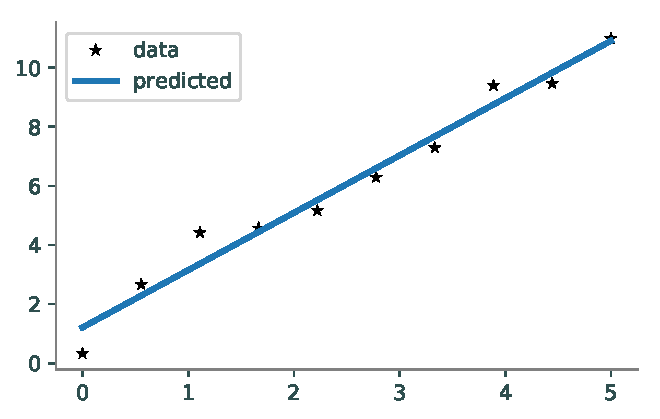
\includegraphics[width=.7\textwidth]{figures/one_d_linear_regression.pdf}
\end{figure}
\end{info}

\subsection*{Transformers} % --------------------------------------------------

A scikit-learn \emph{transformer} processes data to make it better suited for estimation.
This may involve shifting and scaling data, dropping columns, replacing missing values, and so on.

Classes that inherit from the \li{TransformerMixin} base class have a \li{fit()} method that accepts an $N\times D$ matrix $X$ (like an estimator) and an optional set of labels.
The labels are not needed---in fact the \li{fit()} method should do nothing with them---but the parameter for the labels remains as a keyword argument to be consistent with the \li{fit(X,y)} syntax of estimators.
Instead of a \li{predict()} method, the \li{transform()} method accepts data, modifies it (usually via a copy), and returns the result.
The new data may or may not have the same number of columns as the original data.

One common transformation is shifting and scaling the features (columns) so that they each have a mean of 0 and a standard deviation of 1.
The following example implements a basic version of this transformer.

\begin{lstlisting}
>>> from sklearn.base import TransformerMixin

>>> class NormalizingTransformer(BaseEstimator, TransformerMixin):
...     def fit(self, X, y=None):
...         """Calculate the mean and standard deviation of each column."""
...         self.mu_ = np.mean(X, axis=0)
...         self.sig_ = np.std(X, axis=0)
...         return self
...
...     def transform(self, X):
...         """Center each column at zero and normalize it."""
...         return (X - self.mu_) / self.sig_
...
# Fit the transformer and transform the cancer data (both train and test).
>>> nt = NormalizingTransformer()
>>> Z_train = nt.fit_transform(X_train) # Or nt.fit(X_train).transform(X_train)
>>> Z_test = nt.transform(X_test)       # Transform test data (without fitting)

>>> np.mean(Z_train, axis=0)[:3]        # The columns of Z_train have mean 0...
array([-8.08951237e-16, -1.72006384e-17,  1.78678147e-15])
>>> np.std(Z_train, axis=0)[:3]         # ...and have unit variance.
array([1., 1., 1.])
>>> np.mean(Z_test, axis=0)[:3]         # The columns of Z_test each have mean
array([-0.02355067,  0.11665332, -0.03996177])                  # close to 0...
>>> np.std(Z_test, axis=0)[:3]          # ...and have close to unit deviation.
array([0.9263711 , 1.18461151, 0.91548103])

# Check to see if the classification improved.
>>> knn.fit(X_train, y_train).score(X_test, y_test)             # Old score.
0.8951048951048951
>>> knn.fit(Z_train, y_train).score(Z_test, y_test)             # New score.
0.958041958041958
\end{lstlisting}

This particular transformer is implemented as \li{sklearn.preprocessing.StandardScaler}.
A close cousin is \li{sklearn.preprocessing.RobustScaler}, which ignores outliers when choosing the scaling and shifting factors.

Like estimators, transformers may have both hyperparameters (provided to the constructor) and model parameters (determined by \li{fit()}).
Thus a transformer looks and acts like an estimator, with the exception of the \li{predict()} and \li{transform()} methods.

\begin{warn}
The \li{transform()} method should only rely on model parameters derived from the training data in \li{fit()}, \textbf{not} on the data that is worked on in \li{transform()}.
For example, if the \li{NormalizingTransformer} is fit with the input $\widehat{X}$, then \li{transform()} should shift and scale any input $X$ by the mean and standard deviation of $\widehat{X}$, not by the mean and standard deviation of $X$.
Otherwise, the transformation is different for each input $X$.
\end{warn}

\begin{table}[H]
\begin{tabular}{r|l|l}
Scikit-learn Module & \textbf{Classifier} Name & Notable Hyperparameters \\ \hline
\li{discriminant_analysis} & \li{LinearDiscriminantAnalysis} & \li{solver}, \li{shrinkage}, \li{n_components} \\
\li{discriminant_analysis} & \li{QuadraticDiscriminantAnalysis} & \li{reg_param} \\
\li{ensemble} & \li{AdaBoostClassifier} & \li{n_estimators}, \li{learning_rate} \\
% \li{ensemble} & \li{ExtraTreesClassifier} & \li{n_estimators}, \li{max_depth} \\
% \li{ensemble} & \li{GradientBoostingClassifier} & \li{n_estimators}, \li{max_depth} \\
\li{ensemble} & \li{RandomForestClassifier} & \li{n_estimators}, \li{max_depth}\\
\li{linear_model} & \li{LogisticRegression} & \li{penalty}, \li{C} \\
\li{linear_model} & \li{SGDClassifier} & \li{loss}, \li{penalty}, \li{alpha} \\
% \li{naive_bayes} & \li{BernoulliNB} & \li{alpha}, \li{binarize}\\
\li{naive_bayes} & \li{GaussianNB} & \li{priors} \\
\li{naive_bayes} & \li{MultinomialNB} & \li{alpha} \\
\li{neighbors} & \li{KNeighborsClassifier} & \li{n_neighbors}, \li{weights} \\
\li{neighbors} & \li{RadiusNeighborsClassifier} & \li{radius}, \li{weights} \\
\li{neural_network} & \li{MLPClassifier} & \li{hidden_layer_size}, \li{activation} \\
\li{svm} & \li{SVC} & \li{C}, \li{kernel} \\
\li{tree} & \li{DecisionTreeClassifier} & \li{max_depth} \\
& & \\
Scikit-learn Module & \textbf{Regressor} Name & Notable Hyperparameters \\ \hline
\li{ensemble} & \li{AdaBoostRegressor} & \li{n_estimators}, \li{learning_rate} \\
\li{ensemble} & \li{ExtraTreesRegressor} & \li{n_estimators}, \li{max_depth} \\
\li{ensemble} & \li{GradientBoostingRegressor} & \li{n_estimators}, \li{max_depth} \\
\li{ensemble} & \li{RandomForestRegressor} & \li{n_estimators}, \li{max_depth} \\
\li{isotonic} & \li{IsotonicRegression} & \li{y_min}, \li{y_max} \\
\li{kernel_ridge} & \li{KernelRidge} & \li{alpha}, \li{kernel} \\
\li{linear_model} & \li{LinearRegression} & \li{fit_intercept} \\
% \li{neighbors} & \li{KNeighborsRegressor} & \li{n_neighbors}, \li{weights} \\
% \li{neighbors} & \li{RadiusNeighborsRegressor} & \li{radius} \\
\li{neural_network} & \li{MLPRegressor} & \li{hidden_layer_size}, \li{activation} \\
\li{svm} & \li{SVR} & \li{C}, \li{kernel} \\
\li{tree} & \li{DecisionTreeRegressor} & \li{max_depth} \\
& & \\
Module & \textbf{Transformer} Name & Notable Hyperparameters \\ \hline
\li{decomposition} & \li{PCA} & \li{n_components} \\
\li{preprocessing} & \li{Imputer} & \li{missing_values}, \li{strategy} \\
\li{preprocessing} & \li{MinMaxScaler} & \li{feature_range}\\
\li{preprocessing} & \li{OneHotEncoder} & \li{categorical_features}\\
\li{preprocessing} & \li{QuantileTransformer} & \li{n_quantiles}, \li{output_distribution} \\
\li{preprocessing} & \li{RobustScaler} & \li{with_centering}, \li{with_scaling}\\
\li{preprocessing} & \li{StandardScaler} & \li{with_mean}, \li{with_std}\\
\end{tabular}
\caption{Common scikit-learn classifiers, regressors, and transformers.
For full documentation on these classes, see \url{http://scikit-learn.org/stable/modules/classes.html}.}
\end{table}

\section*{Validation Tools} % =================================================

Knowing how to determine whether or not an estimator performs well is an essential part of machine learning.
This often turns out to be a surprisingly sophisticated issue that largely depends on the type of problem being solved and the kind of data that is available for training.
Scikit-learn has validation tools for many situations; for brevity, we restrict our attention to the simple (but important) case of \emph{binary classification}, where the range of the desired model is $Y = \{0,1\}$.

\subsection*{Evaluation Metrics} % --------------------------------------------

The \li{score()} method of a scikit-learn estimator representing the model $f:X\rightarrow\{0,1\}$ returns the \emph{accuracy} of the model, which is the percent of labels that are predicted correctly.
However, accuracy isn't always the best measure of success.
Consider the \emph{confusion matrix} for a classifier, the matrix where the $(i,j)$th entry is the number of observations with actual label $i$ but that are classified as label $j$.
In binary classification, calling the class with label $0$ the \emph{negatives} and the class with label $1$ the \emph{positives}, this becomes the following.

\begin{align*}
\begin{blockarray}{ccc}
& \textrm{Predicted: }0 & \textrm{Predicted: }1 \\
\begin{block}{c[cc]}
\textrm{Actual: }0 & \textrm{True Negatives } (TN) & \textrm{False Positives } (FP)\\
\textrm{Actual: }1 & \textrm{False Negatives } (FN) & \textrm{True Positives } (TP)\\
\end{block}\end{blockarray}
\end{align*}

With this terminology, we define the following metrics.
\begin{itemize}
\item \emph{Accuracy}: $\dfrac{TN + TP}{TN + FN + FP + TP}$, the percent of labels predicted correctly.
\item \emph{Precision}: $\dfrac{TP}{TP + FP}$, the percent of predicted positives that are actually correct.
% This metric indicates how many of the actual positives are classified correctly, and is therefore useful in situations where false positives are dangerous or costly.

\item \emph{Recall}: $\dfrac{TP}{TP + FN}$, the percent of actual positives that are predicted correctly.
\end{itemize}

Precision is useful in situations where false positives are dangerous or costly, while recall is important when avoiding false negatives takes priority.
For example, an email spam filter should avoid filtering out an email that isn't actually spam, so precision is a valuable metric for the filter.
On the other hand, recall is more important in disease detection: it is better to test positive and not have the disease than to test negative when the disease is actually present.
Focusing on a single metric often leads to skewed results (for example, always predicting the same label), so the following metric is also common.
\begin{itemize}
\item \emph{$F_\beta$ Score}: $(1 + \beta^2)
\dfrac{\text{precision}\cdot\text{recall}}{(\beta^2\cdot\text{precision}) + \text{recall}} = \dfrac{(1 + \beta^2)TP}{(1+\beta^2)TP + FP + \beta^2 FN}$.
\end{itemize}

Choosing $\beta < 1$ weighs precision more than recall, while $\beta > 1$ prioritizes recall over precision.
The choice of $\beta = 1$ yields the common $F_1$ score, which weighs precision and recall equally.
This is an important alternative to accuracy when, for example, the training set is heavily unbalanced with respect to the class labels.

Scikit-learn implements these metrics in \li{sklearn.metrics}, as well as functions for evaluating regression, non-binary classification, and clustering models.
The general syntax for such functions is \li{some_score(actual_labels, predicted_labels)}.
For the complete list and further discussion, see \url{http://scikit-learn.org/stable/modules/model_evaluation.html}.

\begin{lstlisting}
>>> from sklearn.metrics import (confusion_matrix, classification_report,
...                              accuracy_score, precision_score,
...                              recall_score, f1_score)

# Fit the esimator to training data and predict the test labels.
>>> knn.fit(X_train, y_train)
>>> knn_predicted = knn.predict(X_test)

# Compute the confusion matrix by comparing actual labels to predicted labels.
>>> CM = confusion_matrix(y_test, knn_predicted)
>>> CM
array([[44,  5],
       [10, 84]])

# Get accuracy (the "usual" score), precision, recall, and f1 scores.
>>> accuracy_score(y_test, knn_predicted)   # (CM[0,0] + CM[1,1]) / CM.sum()
0.8951048951048951
>>> precision_score(y_test, knn_predicted)  # CM[1,1] / CM[:,1].sum()
0.9438202247191011
>>> recall_score(y_test, knn_predicted)     # CM[1,1] / CM[1,:].sum()
0.8936170212765957
>>> f1_score(y_test, knn_predicted)
0.9180327868852459

# Get all of these scores at once with classification_report().
>>> print(classification_report(y_test, knn_predicted))
<<            precision    recall  f1-score   support

           0       0.81      0.90      0.85        49
           1       0.94      0.89      0.92        94

   micro avg       0.90      0.90      0.90       143
   macro avg       0.88      0.90      0.89       143
weighted avg       0.90      0.90      0.90       143>>
\end{lstlisting}

\subsection*{Cross Validation} % ----------------------------------------------

The \li{sklearn.model_selection} module has utilities to streamline and improve model evaluation.

\begin{itemize}
    \item \li{train_test_split()} randomly splits data into training and testing sets (we already used this).
    \item \li{cross_val_score()} randomly splits the data and trains and scores the model a set number of times.
    Each trial uses different training data and results in a different model.
    The function returns the score of each trial.
    \item \li{cross_validate()} does the same thing as \li{cross_val_score()}, but it also reports the time it took to fit, the time it took to score, and the scores for the test set as well as the training set.
\end{itemize}
%
Doing multiple evaluations with different testing and training sets is extremely important.
If the scores on a cross validation test vary wildly, the model is likely overfitting to the training data.

\begin{lstlisting}
>>> from sklearn.model_selection import cross_val_score, cross_validate

# Make (but do not train) a classifier to test.
>>> knn = KNeighborsClassifier(n_neighbors=3)

# Test the classifier on the training data 4 times.
>>> cross_val_score(knn, X_train, y_train, cv=4)
array([0.88811189, 0.92957746, 0.96478873, 0.92253521])

# Get more details on the train/test procedure.
>>> cross_validate(knn, X_train, y_train, cv=4,
...                return_train_score=False)
<<{'fit_time': array([0.00064683, 0.00042295, 0.00040913, 0.00040436]),
 'score_time': array([0.00115728, 0.00109601, 0.00105286, 0.00102782]),
 'test_score': array([0.88811189, 0.92957746, 0.96478873, 0.92253521])}>>

# Do the scoring with an alternative metric.
>>> cross_val_score(knn, X_train, y_train, scoring="f1", cv=4)
array([0.93048128, 0.95652174, 0.96629213, 0.93103448])
\end{lstlisting}

\begin{info}
Any estimator, even a user-defined class, can be evaluated with the scikit-learn tools presented in this section as long as that class conforms to the scikit-learn API discussed previously (i.e., inheriting from the correct base classes, having \li{fit()} and \li{predict()} methods, managing hyperparameters and parameters correctly, and so on).
Any time you define a custom estimator, following the scikit-learn API gives you instant access to tools such as \li{cross_val_score()}.
% This is a huge advantage to understanding the details of the scikit-learn API is the ability to use the validation and training tools to built-in and custom estimators.
\end{info}

\begin{comment} % Further split the training data for validation...
\begin{info}
One way to avoid overfitting is to further split the training set into...

\begin{lstlisting}
# Split the data again.
>>> _, X_val, _, y_val = train_test_split(X_train, y_train)
>>> print(X_train.shape, X_val.shape, X_test.shape)
(319, 30) (80, 30) (143, 30)

# Do a grid search on just the "validation" sets.
>>> param_grid = {"n_neighbors": [2,3,4,5,6],
...               "weights": ["uniform", "distance"]}
>>> knn_gs = GridSearchCV(knn, param_grid, cv=3, scoring="recall")
>>> knn_gs.fit(X_val, y_val)
>>> knn = knn_gs.best_estimator_.fit(X_train, y_train)
>>> print(classification_report(y_test, knn.predict(X_test)))

TODO
\end{lstlisting}
\end{info}
\end{comment}

\subsection*{Grid Search} % ---------------------------------------------------

Recall that the \emph{hyperparameters} of a machine learning model are user-provided parameters that do not depend on the training data.
Finding the optimal hyperparameters for a given model is a challenging and active area of research.\footnote{Intelligent hyperparameter selection is sometimes called \emph{metalearning}.
See, for example, \cite{schoenfeld2018preprocessor}.}
However, brute-force searching over a small hyperparameter space is simple in scikit-learn: a \li{sklearn.model_selection.GridSearchCV} object is initialized with an estimator, a dictionary of hyperparameters, and cross validation parameters (such as \li{cv} and \li{scoring}).
When its \li{fit()} method is called, it does a cross validation test on the given estimator with every possible hyperparameter combination.

For example, a $k$-neighbors classifier has a few important hyperparameters that can have a significant impact on the speed and accuracy of the model: \li{n_neighbors}, the number of nearest neighbors allowed to vote; and \li{weights}, which specifies a strategy for weighting the distances between points.
The following code tests various combinations of these hyperparameters.

\begin{lstlisting}
>>> from sklearn.model_selection import GridSearchCV

>>> knn = KNeighborsClassifier()
# Specify the hyperparameters to vary and the possible values they should take.
>>> param_grid = {"n_neighbors": [2, 3, 4, 5, 6],
...               "weights": ["uniform", "distance"]}
>>> knn_gs = GridSearchCV(knn, param_grid, cv=4, scoring="f1", verbose=1)
>>> knn_gs.fit(X_train, y_train)
<<Fitting 4 folds for each of 5 candidates, totalling 20 fits>>
<r<[Parallel(n_jobs=1)]: Using backend SequentialBackend with 1 concurrent worker.
[Parallel(n_jobs=1)]: Done  20 out of  20 | elapsed:    0.1s finished>r>

# After fitting, the gridsearch object has data about the results.
>>> print(knn_gs.best_params_, knn_gs.best_score_)
<<{'n_neighbors': 5, 'weights': 'uniform'} 0.9532526583188765>>
\end{lstlisting}

The cost of a grid search rapidly increases as the hyperparameter space grows. However, the outcomes of each trial are completely independent of each other, so the problem of training each classifier is \emph{embarassingly parallel}.
To parallelize the grid search over $n$ cores, set the \li{n_jobs} parameter to $n$, or set it to $-1$ to divide the labor between as many cores as are available.

In some circumstances, the parameter grid can be also organized in a way that eliminates redundancy.
Consider an \li{SVC} classifier from \li{sklearn.svm}, an estimator that works by lifting the data into a high-dimensional space, then constructing a hyperplane to separate the classes.
The \li{SVC} has a hyperparameter, \li{kernel}, that determines how the lifting into higher dimensions is done, and for each choice of kernel there are additional corresponding hyperparameters.
To search the total hyperparameter space without redundancies, enter the parameter grid as a list of dictionaries, each of which defines a different section of the hyperparameter space.
In the following code, doing so reduces the number of trials from $3\times 2 \times 3\times 4 = 72$ to only $1 + (1\times 1\times 3) + (1\times 4) = 11$.

\begin{lstlisting}
>>> from sklearn.svm import SVC

>>> svc = SVC(C=0.01, max_iter=100)
>>> param_grid = [
...     {"kernel": ["linear"]},
...     {"kernel": ["poly"], "degree": [2,3], "coef0": [0,1,5]},
...     {"kernel": ["rbf"], "gamma": [.01, .1, 1, 100]}]
>>> svc_gs = GridSearchCV(svc, param_grid,
                          cv=4, scoring="f1",
                          verbose=1, n_jobs=-1).fit(X_train, y_train)
<<Fitting 4 folds for each of 11 candidates, totalling 44 fits>>
<r<[Parallel(n_jobs=-1)]: Using backend LokyBackend with 8 concurrent workers.
[Parallel(n_jobs=-1)]: Done  44 out of  44 | elapsed:    2.4s finished>r>

>>> print(svc_gs.best_params_, svc_gs.best_score_)
<<{'gamma': 0.01, 'kernel': 'rbf'} 0.8909310239174055>>
\end{lstlisting}

See \url{https://scikit-learn.org/stable/modules/grid_search.html} for more details about \li{GridSearchCV} and its relatives.

\section*{Pipelines} % ========================================================

Most machine learning problems require at least a little data preprocessing before estimation in order to get good results.
A scikit-learn \emph{pipeline} (\li{sklearn.pipeline.Pipeline}) chains together one or more transformers and one estimator into a single object, complete with \li{fit()} and \li{predict()} methods.
For example, it is often a good idea to shift and scale data before feeding it into a classifier.
The \li{StandardScaler} transformer can be combined with a classifier with a pipeline.
Calling \li{fit()} on the resulting object calls \li{fit_transform()} on each successive transformer, then \li{fit()} on the estimator at the end.
Likewise, calling \li{predict()} on the \li{Pipeline} object calls \li{transform()} on each transformer, then \li{predict()} on the estimator.

\begin{lstlisting}
>>> from sklearn.preprocessing import StandardScaler
>>> from sklearn.pipeline import Pipeline

# Chain together a scaler transformer and a KNN estimator.
>>> pipe = Pipeline([("scaler", StandardScaler()),      # "scaler" is a label.
                     ("knn", KNeighborsClassifier())])  # "knn" is a label.
>>> pipe.fit(X_train, y_train)
>>> pipe.score(X_test, y_test)
0.972027972027972                       # Already an improvement!
\end{lstlisting}

Since \li{Pipeline} objects behaves like estimators (following the \li{fit()} and \li{predict()} conventions), they can be used with tools like \li{cross_val_score()} and \li{GridSearchCV}.
To specify which hyperparameters belong to which steps of the pipeline, precede each hyperparameter name with \li{<stepname>__}.
For example, \li{knn__n_neighbors} corresponds to the \li{n_neighbors} hyperparameter of the part of the pipeline that is labeled \li{knn}.

\begin{lstlisting}
# Specify the possible hyperparameters for each step.
>>> pipe_param_grid = {"scaler__with_mean": [True, False],
...                    "scaler__with_std": [True, False],
...                    "knn__n_neighbors": [2,3,4,5,6],
...                    "knn__weights": ["uniform", "distance"]}

# Pass the Pipeline object to the GridSearchCV and fit it to the data.
>>> pipe = Pipeline([("scaler", StandardScaler()),
                     ("knn", KNeighborsClassifier())])
>>> pipe_gs = GridSearchCV(pipe, pipe_param_grid,
...                        cv=4, n_jobs=-1, verbose=1).fit(X_train, y_train)
<<Fitting 4 folds for each of 40 candidates, totalling 160 fits>>
<r<[Parallel(n_jobs=-1)]: Using backend LokyBackend with 8 concurrent workers.
[Parallel(n_jobs=-1)]: Done 160 out of 160 | elapsed:    0.3s finished>r>

>>> print(pipe_gs.best_params_, pipe_gs.best_score_, sep='\n')
<<{'knn__n_neighbors': 6, 'knn__weights': 'distance',
 'scaler__with_mean': True, 'scaler__with_std': True}
0.971830985915493>>
\end{lstlisting}

Pipelines can also be used to compare different transformations or estimators.
For example, a pipeline could end in either a \li{KNeighborsClassier()} or an \li{SVC()}, even though they have different hyperparameters.
Like before, use a list of dictionaries to specify the hyperparameter space.

\begin{lstlisting}
>>> pipe = Pipeline([("scaler", StandardScaler()),
                     ("classifier", KNeighborsClassifier())])
>>> pipe_param_grid = [
...     {"classifier": [KNeighborsClassifier()],    # Try a KNN classifier...
...      "classifier__n_neighbors": [2,3,4,5],
...      "classifier__weights": ["uniform", "distance"]},
...     {"classifier": [SVC(kernel="rbf")],         # ...and an SVM classifier.
...      "classifier__C": [.001, .01, .1, 1, 10, 100],
...      "classifier__gamma": [.001, .01, .1, 1, 10, 100]}]
>>> pipe_gs = GridSearchCV(pipe, pipe_param_grid,
...                        cv=5, scoring="f1",
...                        verbose = 1, n_jobs=-1).fit(X_train, y_train)
<<Fitting 5 folds for each of 44 candidates, totalling 220 fits>>
<r<[Parallel(n_jobs=-1)]: Using backend LokyBackend with 8 concurrent workers.
[Parallel(n_jobs=-1)]: Done 220 out of 220 | elapsed:    0.6s finished>r>

>>> params = pipe_gs.best_params_
>>> print("Best classifier:", params["classifier"])
<<Best classifier: SVC(C=10, cache_size=200, class_weight=None, coef0=0.0,
  decision_function_shape='ovr', degree=3, gamma=0.01, kernel='rbf',
  max_iter=-1, probability=False, random_state=None, shrinking=True,
  tol=0.001, verbose=False)>>

# Check the best classifier against the test data.
>>> confusion_matrix(y_test, pipe_gs.predict(X_test))
array([[48,  1],                        # Near perfect!
       [ 1, 93]])
\end{lstlisting}

% Scikit-learn also includes tools for clustering, natural language processing, feature selection, and many, many other machine learning tasks.

\newpage

\section*{Additional Material} % ==============================================

\subsection*{Exercises} % -----------------------------------------------------

\begin{problem} % Write a transformer.
\label{prob:sklearn-custom-clean-titanic}
Writing custom scikit-learn transformers is a convenient way to organize the data cleaning process.
Consider the data in \texttt{titanic.csv}, which contains information about passengers on the maiden voyage of the \emph{RMS Titanic} in 1912.
Write a custom transformer class to clean this data, implementing the \li{transform()} method as follows:
\begin{enumerate}
\item Extract a copy of data frame with just the \li{"Pclass"}, \li{"Sex"}, and \li{"Age"} columns.
\item Replace \li{NaN} values in the \li{"Age"} column (of the copied data frame) with the mean age.
The mean age of the training data should be calculated in \li{fit()} and used in \li{transform()}
(compare this step to using \li{sklearn.preprocessing.Imputer}).
\item Convert the \li{"Pclass"} column datatype to pandas categoricals (\li{pd.CategoricalIndex}).
\item Use \li{pd.get_dummies()} to convert the categorical columns to multiple binary columns (compare this step to using \li{sklearn.preprocessing.OneHotEncoder}).
\item Cast the result as a NumPy array and return it.
\end{enumerate}
Ensure that your transformer matches scikit-learn conventions (it inherits from the correct base classes, \li{fit()} returns \li{self}, etc.).
\end{problem}

\begin{problem} % Use the transformer in an actual prediction.
\label{prob:sklearn-read-and-classify}
Read the data from \texttt{titanic.csv} with \li{pd.read_csv()}.
The \li{"Survived"} column indicates which passengers survived, so the entries of the column are the labels that we would like to predict.
Drop any rows in the raw data that have \li{NaN} values in the \li{"Survived"} column, then separate the column from the rest of the data.
Split the data and labels into training and testing sets.
Use the training data to fit a transformer from Problem \ref{prob:sklearn-custom-clean-titanic}, then use that transformer to clean the training set, then the testing set.
Finally, train a \li{LogisticRegressionClassifier} and a \li{RandomForestClassifier} on the cleaned training data, and score them using the cleaned test set.
\end{problem}

\begin{problem}
Use \li{classification_report()} to score your classifiers from Problem \ref{prob:sklearn-read-and-classify}.
Next, do a grid search for each classifier (using only the cleaned training data), varying at least two hyperparameters for each kind of model.
% Extract the resulting best estimators (the \li{best_estimator_} attribute of the \li{GridSearchCV} object) and refit them to the training data.
Use \li{classification_report()} to score the resulting best estimators with the cleaned test data.
Try changing the hyperparameter spaces or scoring metrics so that each grid search yields a better estimator.
\end{problem}

\begin{problem}
Make a pipeline with at least two transformers to further process the Titanic dataset.
Do a gridsearch on the pipeline and report the hyperparameters of the best estimator.
\end{problem}
